% Options for packages loaded elsewhere
\PassOptionsToPackage{unicode}{hyperref}
\PassOptionsToPackage{hyphens}{url}
%
\documentclass[
]{article}
\usepackage{amsmath,amssymb}
\usepackage{lmodern}
\usepackage{ifxetex,ifluatex}
\ifnum 0\ifxetex 1\fi\ifluatex 1\fi=0 % if pdftex
  \usepackage[T1]{fontenc}
  \usepackage[utf8]{inputenc}
  \usepackage{textcomp} % provide euro and other symbols
\else % if luatex or xetex
  \usepackage{unicode-math}
  \defaultfontfeatures{Scale=MatchLowercase}
  \defaultfontfeatures[\rmfamily]{Ligatures=TeX,Scale=1}
\fi
% Use upquote if available, for straight quotes in verbatim environments
\IfFileExists{upquote.sty}{\usepackage{upquote}}{}
\IfFileExists{microtype.sty}{% use microtype if available
  \usepackage[]{microtype}
  \UseMicrotypeSet[protrusion]{basicmath} % disable protrusion for tt fonts
}{}
\makeatletter
\@ifundefined{KOMAClassName}{% if non-KOMA class
  \IfFileExists{parskip.sty}{%
    \usepackage{parskip}
  }{% else
    \setlength{\parindent}{0pt}
    \setlength{\parskip}{6pt plus 2pt minus 1pt}}
}{% if KOMA class
  \KOMAoptions{parskip=half}}
\makeatother
\usepackage{xcolor}
\IfFileExists{xurl.sty}{\usepackage{xurl}}{} % add URL line breaks if available
\IfFileExists{bookmark.sty}{\usepackage{bookmark}}{\usepackage{hyperref}}
\hypersetup{
  pdftitle={Codebook bundeslaendeR polidoc Link},
  pdfauthor={Robert Stelzle},
  hidelinks,
  pdfcreator={LaTeX via pandoc}}
\urlstyle{same} % disable monospaced font for URLs
\usepackage[margin=1in]{geometry}
\usepackage{graphicx}
\makeatletter
\def\maxwidth{\ifdim\Gin@nat@width>\linewidth\linewidth\else\Gin@nat@width\fi}
\def\maxheight{\ifdim\Gin@nat@height>\textheight\textheight\else\Gin@nat@height\fi}
\makeatother
% Scale images if necessary, so that they will not overflow the page
% margins by default, and it is still possible to overwrite the defaults
% using explicit options in \includegraphics[width, height, ...]{}
\setkeys{Gin}{width=\maxwidth,height=\maxheight,keepaspectratio}
% Set default figure placement to htbp
\makeatletter
\def\fps@figure{htbp}
\makeatother
\setlength{\emergencystretch}{3em} % prevent overfull lines
\providecommand{\tightlist}{%
  \setlength{\itemsep}{0pt}\setlength{\parskip}{0pt}}
\setcounter{secnumdepth}{-\maxdimen} % remove section numbering
\usepackage{longtable}
\usepackage{float}
\usepackage{graphicx}
\usepackage{booktabs}
\usepackage{longtable}
\usepackage{array}
\usepackage{multirow}
\usepackage{wrapfig}
\usepackage{float}
\usepackage{colortbl}
\usepackage{pdflscape}
\usepackage{tabu}
\usepackage{threeparttable}
\usepackage{threeparttablex}
\usepackage[normalem]{ulem}
\usepackage{makecell}
\usepackage{xcolor}
\ifluatex
  \usepackage{selnolig}  % disable illegal ligatures
\fi

\title{Codebook bundeslaendeR polidoc Link}
\author{Robert Stelzle}
\date{21.01.2022}

\begin{document}
\maketitle

\hypertarget{link_polidoc_parties-and-link_polidoc_governments}{%
\subsection{\texorpdfstring{\texttt{link\_polidoc\_parties} and
\texttt{link\_polidoc\_governments}}{link\_polidoc\_parties and link\_polidoc\_governments}}\label{link_polidoc_parties-and-link_polidoc_governments}}

\texttt{link\_polidoc\_parties} and \texttt{link\_polidoc\_governments}
provide easy links of either \texttt{ltw\_election\_results} or
\texttt{ltw\_election\_results\_and\_gov} with party manifestos and
coalition agreements made available from polidoc.net - The Political
Documents Archive. While file names from polidoc.net follow a naming
pattern (\{partyID\}.\{stateID\}.\{year\}.\{1\}.\{number of party
manifesto for election\}), the provided links make joining the data
easier.

Note that polidoc.net provides a manifesto for the Neue Liberale in the
HB 2015 election (41441.005.2015.1.1). Since the party withdrew it's
candidacy before the election and is thus not included in the election
results in \texttt{ltw\_election\_results}, the manifesto id is not
included in link\_polidoc\_parties.

Note that polidoc.net provides a coalition agreement between the SPD and
the Greens following the 2008 HE election (41001.006.2008.1.1). Since
this potential coalition under leadership of SPD politician Andrea
Ypsilanti never came to be due to several SPD MPs opposing the red-green
minority cabinet being externally supported by Die Linke the coalition
agreement can't be matched with a government in
\texttt{ltw\_election\_results\_and\_gov} and is thus not included.

\newpage

\hypertarget{variables}{%
\section{Variables}\label{variables}}

\begin{longtable}{p{3.2cm}| p{11cm}}
\texttt{state} &\textbf{State Abbreviation}\newline 
ISO 3166-2:DE-code of the state;
           including BA for the former state of Baden, WH for the former state
           of Württemberg-Hohenzollern and WB for the former state of
           Württemberg-Baden.
\end{longtable}

\begin{longtable}{p{3.2cm}| p{11cm}}
\texttt{election\_date} &\textbf{Election Date}\newline 
Date of the election.  ISO 8601 or R-Date format.
\end{longtable}

\begin{longtable}{p{3.2cm}| p{11cm}}
\texttt{polidoc\_filename and polidoc\_filename\_2 in link\_polidoc\_
parties} &\textbf{Polidoc File Name of Party Manifesto}\newline 
File name of state party manifesto (or 2nd manifesto if available) available in The Political Documents Archive (polidoc.net).


\hspace*{.25cm}
\begin{minipage}[t]{\linewidth }
\vspace{0pt}
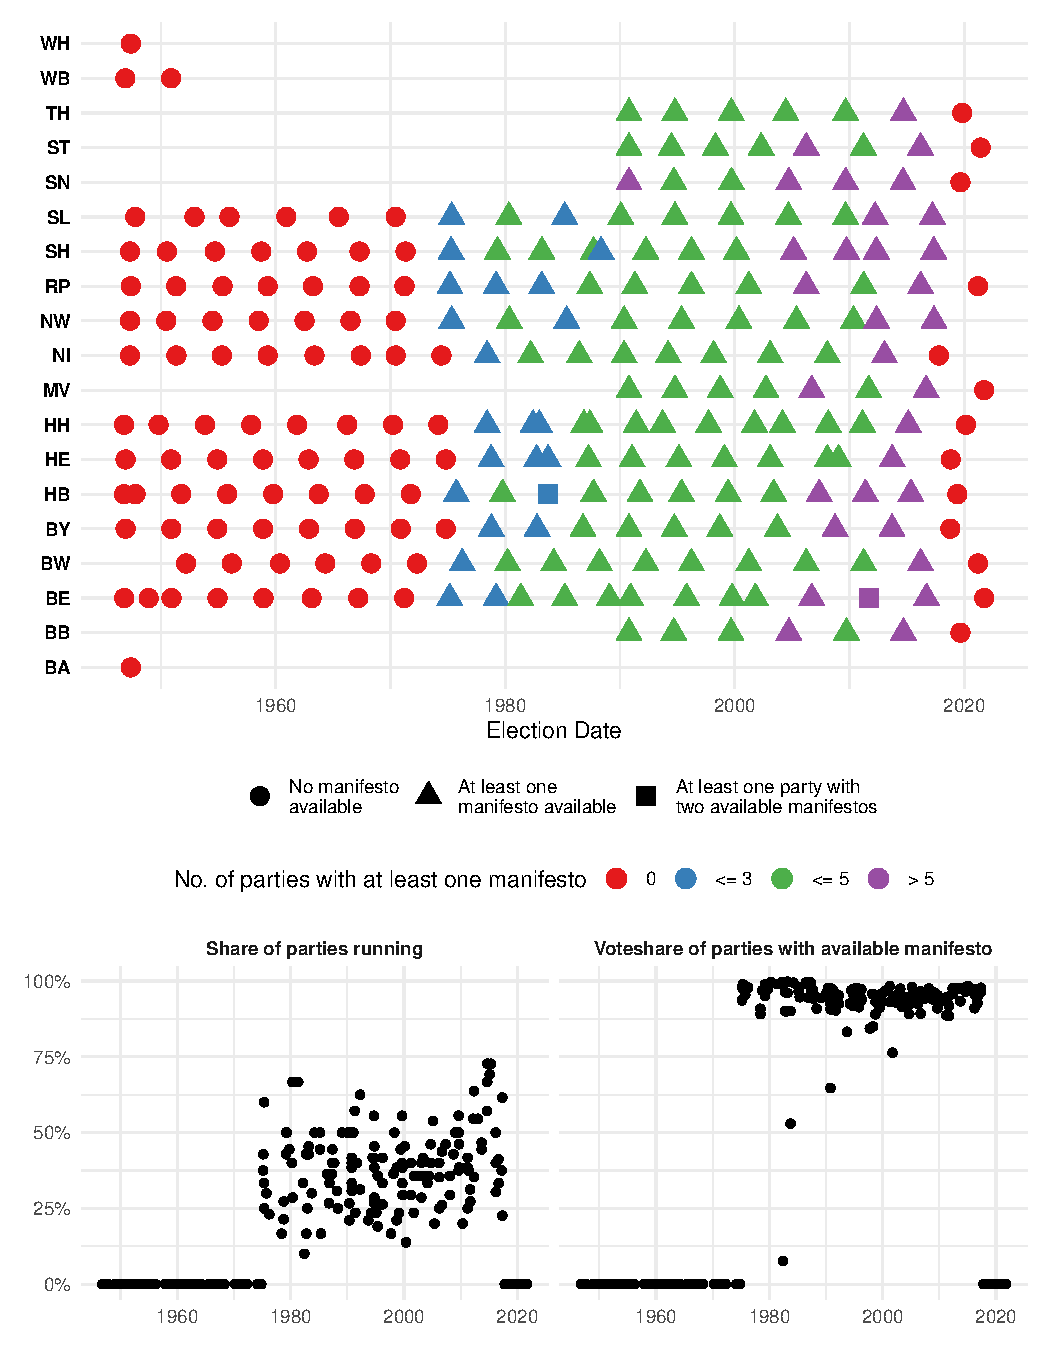
\includegraphics[width = \linewidth]{cbpolidoc/pltpolidocparties.pdf}
\end{minipage}


\end{longtable}

\begin{longtable}{p{3.2cm}| p{11cm}}
\texttt{polidoc\_filename in link\_polidoc\_
governments} &\textbf{Polidoc File Name of Coalition Agreement}\newline 
File name of coalition agreement available in The Political Documents Archive (polidoc.net).


\hspace*{.25cm}
\begin{minipage}[t]{\linewidth }
\vspace{0pt}
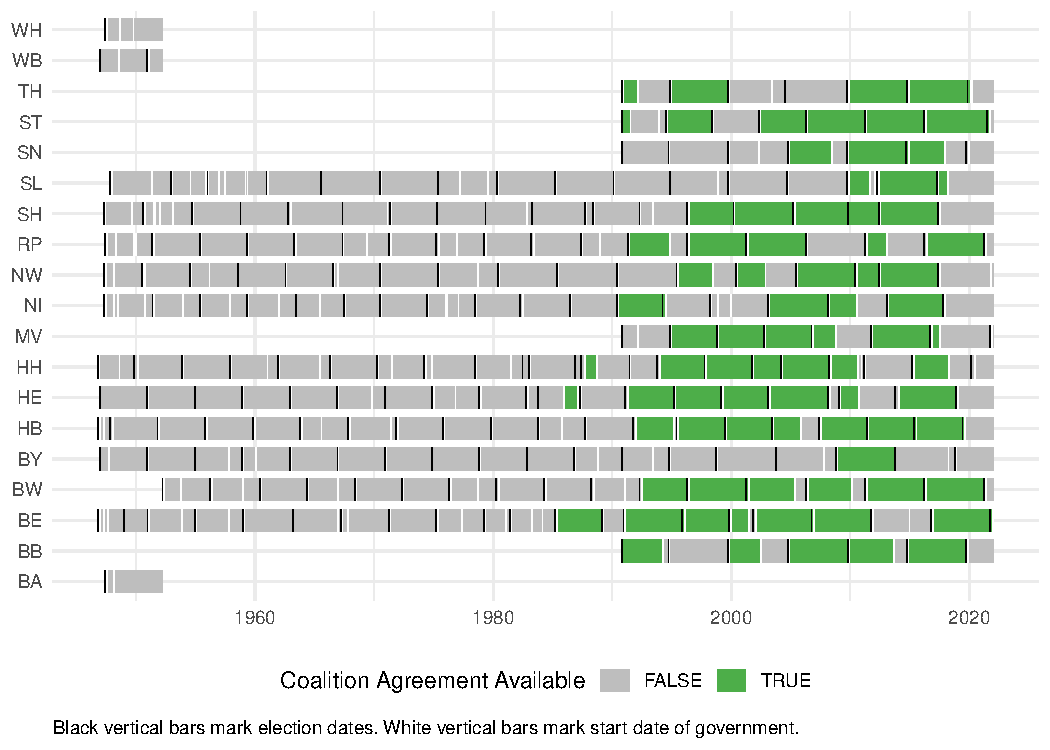
\includegraphics[width = \linewidth]{cbpolidoc/pltpolidocgov.pdf}
\end{minipage}





\end{longtable}

\end{document}
